\documentclass[11pt,a4paper]{article}
\usepackage[T1]{fontenc}
\usepackage{lmodern}
\usepackage[margin=2.2cm]{geometry}
\usepackage{amsmath,amssymb}
\usepackage{booktabs,tabularx,array}
\usepackage{graphicx}
\usepackage{float}
\usepackage{longtable}
\usepackage{xcolor}
\usepackage{tikz}
\usetikzlibrary{arrows.meta,positioning}
\usepackage[hidelinks]{hyperref}
\def\sectionautorefname{Section}\def\subsectionautorefname{Section}

\definecolor{navy}{HTML}{1F3A5F}
\definecolor{soft}{HTML}{EEF3FA}
\definecolor{todo}{HTML}{FDF1E9}
\definecolor{todoline}{HTML}{EB6834}
\newcommand{\code}[1]{\texttt{\small #1}}
% A box the author fills in: the course does not allow LLM-written analysis or conclusions.
\newcommand{\authorbox}[2]{\par\smallskip\noindent\fcolorbox{todoline}{todo}{\parbox{\dimexpr\linewidth-2\fboxsep-2\fboxrule}{%
  \small\textbf{To be written by the author --- #1}\par\smallskip #2}}\par\smallskip}

% generated by make_figures.py
\newcommand{\docsDissent}{2}
\newcommand{\docsOverruled}{1}
\newcommand{\ensCthree}{0.511}
\newcommand{\ensCthreecal}{0.512}
\newcommand{\goldseg}{28.2}
\newcommand{\kdparams}{62.9M}
\newcommand{\ndocsCL}{45}
\newcommand{\ndocsIT}{45}
\newcommand{\nzips}{35}
\newcommand{\oofEeight}{0.326}
\newcommand{\oofEfive}{0.423}
\newcommand{\oofEfour}{0.406}
\newcommand{\oofEnine}{0.272}
\newcommand{\oofEone}{0.455}
\newcommand{\oofEoneorig}{0.427}
\newcommand{\oofEseven}{0.396}
\newcommand{\oofEsix}{0.403}
\newcommand{\oofEthree}{0.441}
\newcommand{\oofEtwo}{0.330}
\newcommand{\oofEzero}{0.361}
\newcommand{\oofTeight}{0.491}
\newcommand{\oofTfour}{0.477}
\newcommand{\oofTnine}{0.466}
\newcommand{\oofTone}{0.416}
\newcommand{\oofToneeight}{0.500}
\newcommand{\oofTonefive}{0.493}
\newcommand{\oofTonefour}{0.501}
\newcommand{\oofTonenine}{0.500}
\newcommand{\oofToneone}{0.447}
\newcommand{\oofToneseven}{0.500}
\newcommand{\oofTonesix}{0.497}
\newcommand{\oofTonethree}{0.498}
\newcommand{\oofTonetwo}{0.422}
\newcommand{\oofTonezero}{0.485}
\newcommand{\oofTseven}{0.500}
\newcommand{\oofTsix}{0.459}
\newcommand{\oofTthree}{0.467}
\newcommand{\oofTtwo}{0.459}
\newcommand{\persistCL}{0.94}
\newcommand{\persistIT}{0.75}
\newcommand{\predseg}{32.5}
\newcommand{\sentsOverruled}{3}
\newcommand{\simmean}{0.585}
\newcommand{\simpninety}{0.649}
\newcommand{\simpten}{0.522}
\newcommand{\teacherparams}{90.3M}
\newcommand{\topconf}{Ratio$\to$PrecRelied 548; PrecRelied$\to$Ratio 539; Fact$\to$Ratio 499; ArgPet$\to$ArgResp 370; ArgResp$\to$ArgPet 367; RulingLower$\to$Ratio 268}

\makeatletter\newcommand{\tabinput}[1]{\@@input #1 }\makeatother % expandable \input inside tabulars

\title{\textbf{CS-781 Capstone, Phase 3: Rhetorical Role Prediction}\\[2pt]
\large A hierarchical sentence tagger on the four Phase-1 language models}
\author{Manish Kumar (251330604)\\ CS-781, IIT Kanpur}
\date{October 2026}

\begin{document}
\maketitle

\begin{abstract}
\noindent Every sentence of a Corporate Law (CL) or Information Technology (IT) judgment is assigned one of
thirteen rhetorical roles.  Labels come in long runs (the next sentence has the same label with probability
\persistCL{} in CL and \persistIT{} in IT), so we build a hierarchical tagger: a Phase-1 language model
encodes windows of neighbouring sentences, each sentence is mean-pooled, a BiLSTM with position and domain
embeddings reads the document, and a sentence-level CRF decodes the label sequence.  All four Phase-1
architectures are adapted with nine techniques (LoRMA+, LoRA, rsLoRA, QLoRA, AdaLoRA, IA$^3$, prefix tuning,
prompt tuning and knowledge distillation), evaluated by five-fold document-level cross-validation over the 90
labelled documents.  The context-free ablation scores \oofEzero{} out-of-fold macro-F1 against \oofEone{} for
the same encoder with context.  A tuning round (causal attention for the decoder backbones, longer training,
weaker logit adjustment) lifts every technique it was applied to, the best single models reaching
\oofTonefour{} (A1 LoRA) and \oofTseven{} (A4 LoRMA+); a four-model ensemble reaches \ensCthree.  All numbers
are generated from the run outputs by \code{p3/report/make\_figures.py}.
\end{abstract}

\tableofcontents
\newpage

% =====================================================================
\section{Introduction}
Rhetorical role (RR) prediction labels each sentence of a judgment with its function: facts, issues, the
arguments of each side, statutes, precedents relied on or not, the lower court's ruling, the ratio of the
decision, the present court's ruling, dissent, or none.  Phase~3 provides judgments from two domains, Corporate
Law (CL) and Information Technology (IT); the prediction must contain exactly one official label per sentence,
in order, and the primary metric is macro-F1 (macro precision and recall are secondary).  The rules require
the Phase-1 models as the only pretrained weights, all four architectures across the submissions, at least six
substantially different experiments of which at least five are different adaptation techniques, LoRMA and
knowledge distillation.

The report covers the data (\autoref{sec:data}), the model and every adaptation method
(\autoref{sec:methods}), the evaluation and submission protocol (\autoref{sec:protocol}), the first round of
experiments (\autoref{sec:res-first}), the tuning rounds (\autoref{sec:res-tune}), per-label and confusion
results (\autoref{sec:res-labels}), and ensembles, calibration and decoding-time post-processing
(\autoref{sec:res-ens}).

% =====================================================================
\section{Data}\label{sec:data}
\begin{table}[H]\centering\small
\caption{Documents and sentences (train + official dev, which we pool for cross-validation). Persistence =
probability that a sentence has the same label as the previous one.}\label{tab:data}
\begin{tabular}{lrrrrrrr}\toprule
Domain & Docs & Sentences & Median sent./doc & Max & Test docs & Test sent. & Persistence\\\midrule
\tabinput{tables/data.tex}
\bottomrule\end{tabular}\end{table}

\begin{figure}[H]\centering
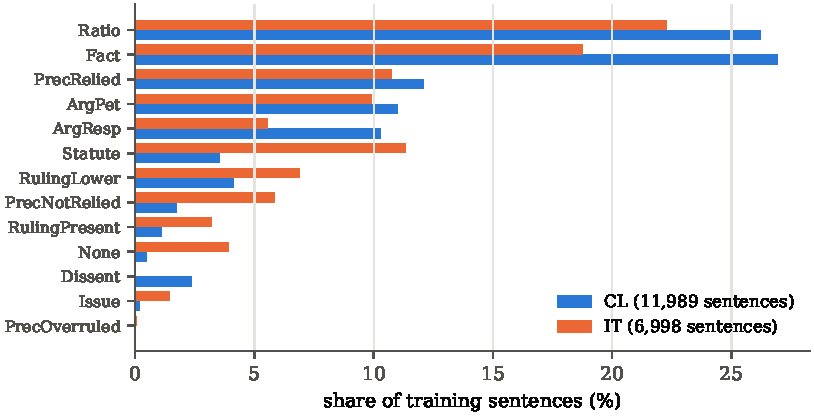
\includegraphics[width=0.85\linewidth]{figs/labels.pdf}
\caption{Label distribution per domain (train + dev).}
\label{fig:labels}\end{figure}

\begin{table}[H]\centering\small
\caption{Sentences per label and domain.}\label{tab:labels}
\begin{tabular}{lrrrr}\toprule
Label & \multicolumn{2}{c}{CL} & \multicolumn{2}{c}{IT}\\\midrule
\tabinput{tables/labels.tex}
\bottomrule\end{tabular}\end{table}
Dissent occurs in \docsDissent{} of the 90 documents and PrecedentOverruled in \docsOverruled{}
(\sentsOverruled{} sentences).

% =====================================================================
\section{Methods}\label{sec:methods}
\subsection{Hierarchical model}
\begin{figure}[H]\centering
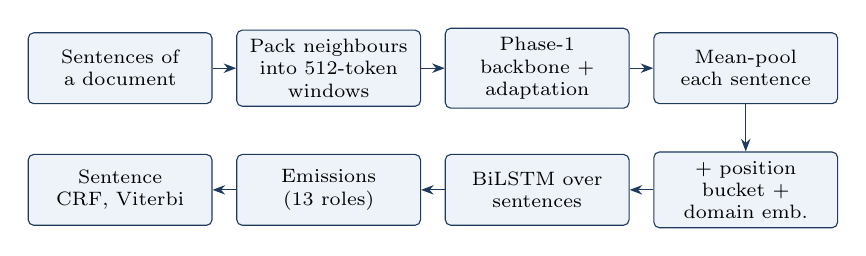
\begin{tikzpicture}[node distance=3mm, box/.style={draw=navy,rounded corners=2pt,fill=soft,align=center,
  font=\scriptsize,minimum height=9mm,text width=21mm}, arr/.style={-{Stealth[length=1.6mm]},navy}]
  \node[box] (a) {Sentences of a document};
  \node[box,right=of a] (b) {Pack neighbours into 512-token windows};
  \node[box,right=of b] (c) {Phase-1 backbone + adaptation};
  \node[box,right=of c] (d) {Mean-pool each sentence};
  \node[box,below=6mm of d] (e) {+ position bucket + domain emb.};
  \node[box,left=of e] (f) {BiLSTM over sentences};
  \node[box,left=of f] (g) {Emissions (13 roles)};
  \node[box,left=of g] (h) {Sentence CRF, Viterbi};
  \foreach \x/\y in {a/b,b/c,c/d,d/e,e/f,f/g,g/h} \draw[arr] (\x)--(\y);
\end{tikzpicture}
\caption{The rhetorical-role model (\code{p3/rr/model.py}).}
\label{fig:model}\end{figure}

\begin{itemize}
  \item \textbf{Sentence encoding with context.} Each sentence (at most 128 tokens; the 95th percentile is
  72--84 words) is tokenized with the Phase-1 BPE as \texttt{" "} + text, and consecutive sentences are packed
  into windows of at most 512 tokens, so every sentence is encoded together with its neighbours.  The ablation
  E0 encodes every sentence alone (\code{data.context: none}).
  \item \textbf{Pooling.} A sentence vector is the mean of its tokens' final hidden states.
  \item \textbf{Document layer.} The vector is projected to 256 dimensions (dropout 0.1, GELU), added to a
  relative-position embedding (sentence index / document length, 20 buckets) and a domain embedding (CL or IT),
  and a one-layer BiLSTM \cite{hochreiter1997lstm} reads the sentences of the document.
  \item \textbf{Output.} A linear layer gives 13 emission scores per sentence; a linear-chain CRF
  \cite{lafferty2001crf} over the sentence sequence learns label transitions and is decoded with Viterbi.
  E0 uses independent softmax decisions instead.
\end{itemize}
The design follows hierarchical BiLSTM-CRF models for rhetorical roles \cite{bhattacharya2019rr,malik2022rr}.

\subsection{Backbones}
The backbone loading and the A2 handling are shared with Phase~2 (\code{p2/lner/backbones.py}): A1 and A4 run
with the Phase-1 causal mask (\code{attention: causal}) or without it (\code{bidirectional}); A3 reads the
whole window as its bidirectional prefix; A2 uses its decoder states (its encoder output is nearly collapsed,
Phase-2 report).  The first-round experiments use bidirectional attention for A1 and A4, as in Phase~2; the
tuning rounds switch them to causal (\autoref{sec:res-tune}).  All experiments start from the cleaned Phase-1
checkpoints (1B tokens); E1 is also run on the original A4 checkpoint.

\subsection{Training}
Each optimizer step accumulates 4 chunks of 128 consecutive sentences (random start per chunk; every
document contributes $\lceil n/128\rceil$ chunks per epoch).  AdamW, learning rate $10^{-3}$ for the adapted
backbone parameters ($3\times10^{-3}$ for IA$^3$ and prompt tuning, $10^{-4}$ for the fully fine-tuned KD
student) and $10^{-3}$ for the document layer, weight decay 0.01, 10\% linear warm-up then cosine decay,
gradient clipping 1.0, bf16.  First round: up to 12 epochs, early stopping after 4 epochs without improvement
on the fold's held-out documents; tuned runs: 20 epochs, patience 6.  The best epoch is kept.

\paragraph{Logit adjustment.} The training loss uses scores $s_y + \tau\log\pi_y$, where $\pi$ is the label
prior of the training folds \cite{menon2021logit}; at inference the raw scores are used.  This raises the
relative score of rare roles, which macro-F1 weights equally.  $\tau=1$ in the first round, $0.5$ after tuning.

\subsection{Adaptation methods}\label{sec:peft}
LoRA, LoRMA+ and IA$^3$ come from Phase~2, in \code{p2/lner/peft.py}.  The other methods are new, in
\code{p3/rr/peft\_extra.py}.  The document layer and CRF are always trained.
\begin{itemize}
  \item \textbf{LoRMA+} \cite{bihany2025lorma}: $W = (I + \frac{\alpha}{r}BA)\,W_0$, computed as
  $h_0=W_0x$, $h=h_0+\frac{\alpha}{r}B(Ah_0)$; $r=16$, $\alpha=32$, on the attention and MLP projections.
  \item \textbf{LoRA} \cite{hu2022lora}: $h = W_0x + \frac{\alpha}{r}BAx$; $r=16$, $\alpha=32$.
  \item \textbf{rsLoRA} \cite{kalajdzievski2023rslora}: LoRA with scale $\alpha/\sqrt{r}$ instead of
  $\alpha/r$, which keeps the update's size stable at high rank; $r=64$, $\alpha=16$.
  \item \textbf{QLoRA} \cite{dettmers2023qlora}: every linear layer of the frozen backbone is stored as 4-bit
  NormalFloat (the 16 quantiles of a standard normal rescaled to $[-1,1]$), with one absmax scale per block of
  64 weights and two 4-bit codes packed per byte; weights are de-quantized on the fly, and LoRA ($r=16$) is
  trained in higher precision on top.  The relative reconstruction error of a Gaussian weight matrix is 9\%,
  and storage is 8$\times$ smaller than fp32.
  \item \textbf{AdaLoRA} \cite{zhang2023adalora}: the update is $P\,\mathrm{diag}(\lambda)\,Q$ with an
  orthogonality penalty $\|P^\top P-I\|^2+\|QQ^\top-I\|^2$ (weight 0.1).  The importance of each singular value
  is its smoothed sensitivity $|w\cdot\nabla w|$ times its uncertainty (EMA factors 0.85), summed over
  $\lambda_i$ and the mean of its column of $P$ and row of $Q$.  The global budget falls cubically from rank 12
  to an average of 8 per module between 10\% and 70\% of training; the lowest-importance singular values are
  masked every 10 steps.
  \item \textbf{IA$^3$} \cite{liu2022ia3}: learned scaling vectors on keys, values and the MLP's inner
  activation, initialised to one.
  \item \textbf{Prefix tuning} \cite{li2021prefix}: 16 learned key/value vectors per self-attention layer,
  produced by a shared two-layer MLP from 16 prefix embeddings (hidden 512, last layer initialised to zero);
  prefix keys carry no rotary position, and every attention mask is extended to let all tokens attend to them.
  \item \textbf{Prompt tuning} \cite{lester2021prompt}: 20 learned input embeddings, initialised from random
  vocabulary embeddings, replace the first 20 positions of every window.
  \item \textbf{Knowledge distillation} \cite{hinton2015kd}: the student is A4 with 6 of its 10 blocks (blocks
  0, 2, 4, 5, 6, 8, which keep all three global-attention layers), \kdparams{} parameters against
  \teacherparams{} for the teacher, fully fine-tuned with
  $\alpha\,\mathcal{L}_\text{task} + (1-\alpha)\,T^2\,\mathrm{KL}(p^T_\text{teacher}\,\|\,p^T_\text{student})$
  on the emission scores, $\alpha=0.5$, $T=2$.  The fold-$k$ student learns from the fold-$k$ teacher, which
  was trained on the same documents.
\end{itemize}

\section{Evaluation and submission protocol}\label{sec:protocol}
\begin{itemize}
  \item \textbf{Cross-validation.} The official dev set has only 5 documents per domain, with a different label
  mix from train (for example ArgumentPetitioner is 9\% of CL train and 25\% of CL dev).  We pool train and dev
  (90 documents) and split them into 5 document-level folds, stratified by domain (\code{cv.seed}=0, the same
  folds for every run).
  \item \textbf{Out-of-fold (OOF) score.} Each document is predicted by the fold model that did not train on it;
  macro-F1 is computed over all 90 documents (labels present in gold or predictions, as in scikit-learn), and
  also per domain.  The mean $\pm$ standard deviation of the five per-fold scores is reported alongside.
  \item \textbf{Submission.} The five fold models score the test documents; their log-softmax emissions and CRF
  parameters are averaged and decoded with Viterbi (\code{make\_submission.py}).  The writer checks that every
  test document is present, with one official label per sentence in order, and puts \code{prediction.json} at
  the root of the zip.
  \item \textbf{Cross-run ensembles} (\code{ensemble\_cv.py}, \code{calibrate.py}): the same averaging over
  several experiments, scored out-of-fold with each fold's models.
  \item \textbf{Calibration} (\code{calibrate.py}): a per-label bias added to the emissions before Viterbi,
  fitted by coordinate ascent over $\{-1,-0.75,\dots,1\}$ to maximise macro-F1 (labels with fewer than 20
  out-of-fold sentences keep zero).  The reported score is nested: for each fold, the bias is fitted on the
  other folds' documents only.
  \item \textbf{Decoding-time post-processing} (\code{postproc.py}): never emitting given labels, and scaling
  the CRF transition scores.  Because a test set has only 10 documents, it is also scored on 3{,}000 simulated
  test sets of 5 CL + 5 IT out-of-fold documents, each scored on its own.
\end{itemize}

% =====================================================================
\section{Results}
\subsection{First round}\label{sec:res-first}
\begin{table}[H]\centering
\caption{First-round experiments: out-of-fold (OOF) macro-F1 over 90 documents, per domain, fold mean $\pm$
std, macro precision / recall, minutes per fold, peak GPU memory (GB), checkpoint (MB).}\label{tab:first}
\resizebox{\linewidth}{!}{\begin{tabular}{lllrrrrrrrrrr}\toprule
Run & Arch & Method & Trainable & OOF F1 & CL & IT & Fold mean & P & R & Min & GB & MB\\\midrule
\tabinput{tables/first.tex}
\bottomrule\end{tabular}}\end{table}

\begin{itemize}
  \item \textbf{Context}: E0 (each sentence alone, no BiLSTM, no CRF) \oofEzero{}; E1 (same encoder and method,
  with context) \oofEone.
  \item \textbf{Phase-1 backbone}: E1 on the original A4 \oofEoneorig; on the cleaned 1B-token A4 \oofEone.
\end{itemize}

\begin{figure}[H]\centering
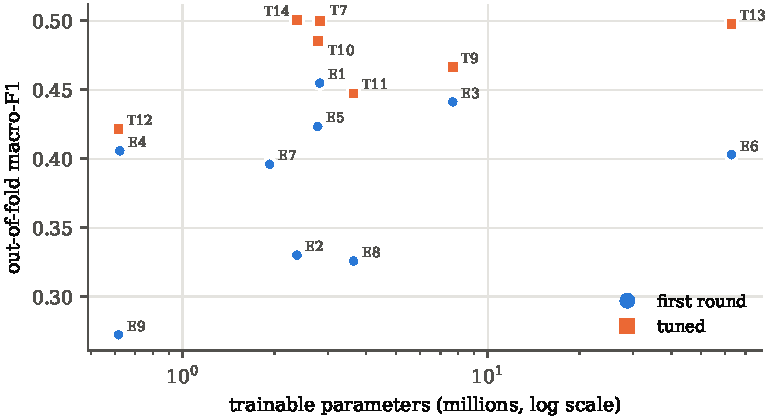
\includegraphics[width=0.82\linewidth]{figs/efficiency.pdf}
\caption{OOF macro-F1 against trained parameters (document layer included), first round and tuned runs.}
\label{fig:eff}\end{figure}

\subsection{Tuning rounds}\label{sec:res-tune}
Four rounds of follow-up runs, each defined by a config that inherits from an earlier experiment.  The
``purpose'' is the comment written in the config before the run; the ``change'' is the computed difference
between the two configs; $\Delta$ is the OOF difference against the parent.

{\scriptsize\setlength{\tabcolsep}{3pt}
\begin{longtable}{llp{5.4cm}p{3.6cm}rrr}\caption{Tuning runs.}\label{tab:tuning}\\\toprule
Run & Parent & Purpose & Change & OOF F1 & $\Delta$ & Fold mean\\\midrule\endfirsthead
\toprule Run & Parent & Purpose & Change & OOF F1 & $\Delta$ & Fold mean\\\midrule\endhead
\tabinput{tables/tuning.tex}
\bottomrule\end{longtable}}

\begin{figure}[H]\centering
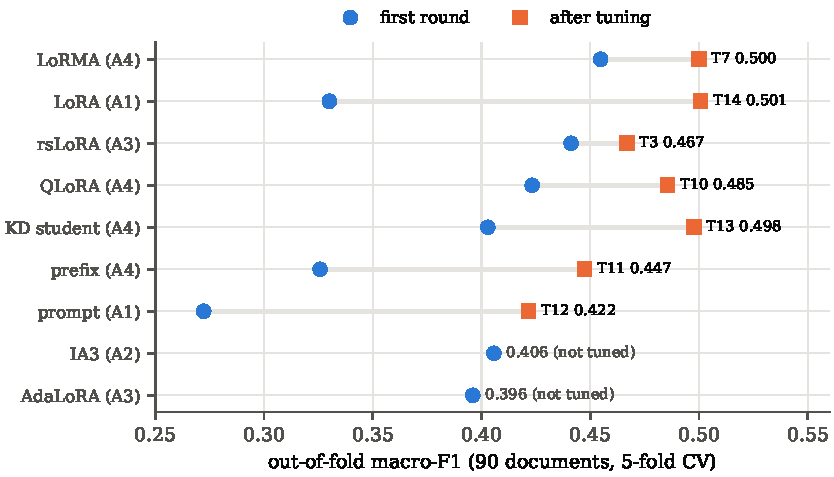
\includegraphics[width=0.85\linewidth]{figs/tuning.pdf}
\caption{Each technique's first-round OOF macro-F1 and its best tuned version.}
\label{fig:tuning}\end{figure}

\subsection{Per-label results and confusions}\label{sec:res-labels}
\begin{figure}[H]\centering
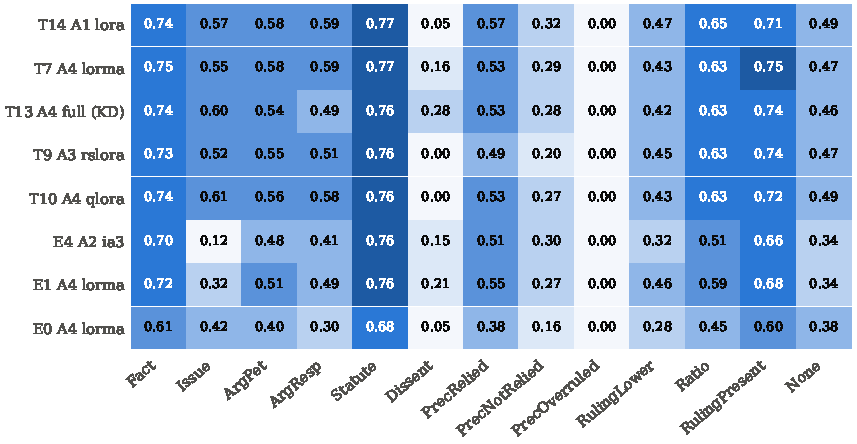
\includegraphics[width=0.95\linewidth]{figs/per_label.pdf}
\caption{OOF F1 per label for the best tuned runs and three first-round references.}
\label{fig:perlabel}\end{figure}

\begin{figure}[H]\centering
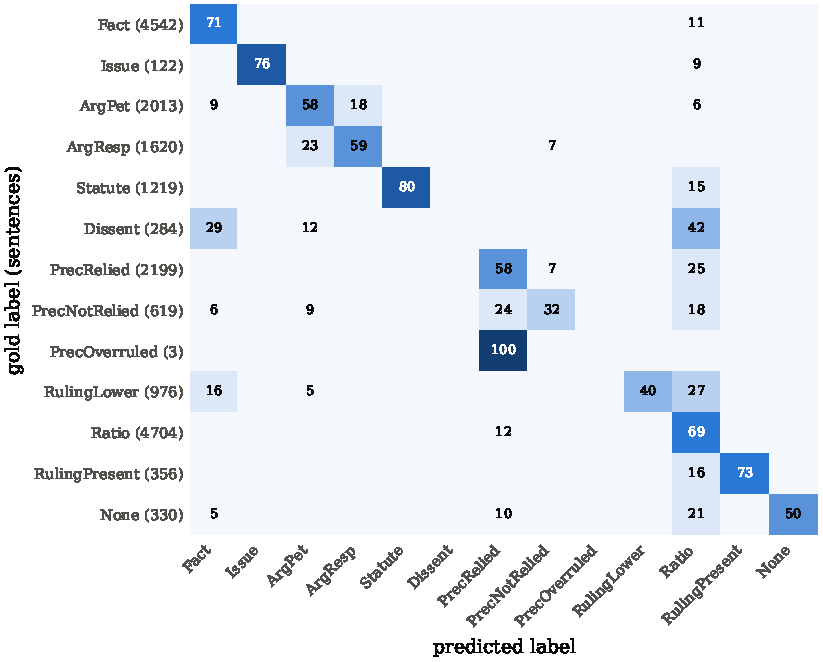
\includegraphics[width=0.72\linewidth]{figs/confusion.pdf}
\caption{Row-normalised OOF confusion matrix of T14 (A1 LoRA), in percent of each gold label; cells below 5\%
are left blank.}
\label{fig:confusion}\end{figure}
Largest confusions in sentences (gold $\to$ predicted, T14): \topconf.

\subsection{Ensembles, calibration and post-processing}\label{sec:res-ens}
\begin{table}[H]\centering\small
\caption{Cross-run ensembles and calibration (OOF macro-F1; calibrated = nested-CV estimate).}\label{tab:ens}
\begin{tabular}{llrrrrr}\toprule
Name & Members & OOF F1 & CL & IT & Calibrated & $\Delta$\\\midrule
\tabinput{tables/ensembles.tex}
\bottomrule\end{tabular}\end{table}

For the C3 ensemble the predicted label sequence has \predseg{} segments per document on average, against
\goldseg{} in gold.  On the simulated 10-document test sets C3 scores \simmean{} on average, with a
10th--90th percentile range of \simpten--\simpninety.

\begin{figure}[H]\centering
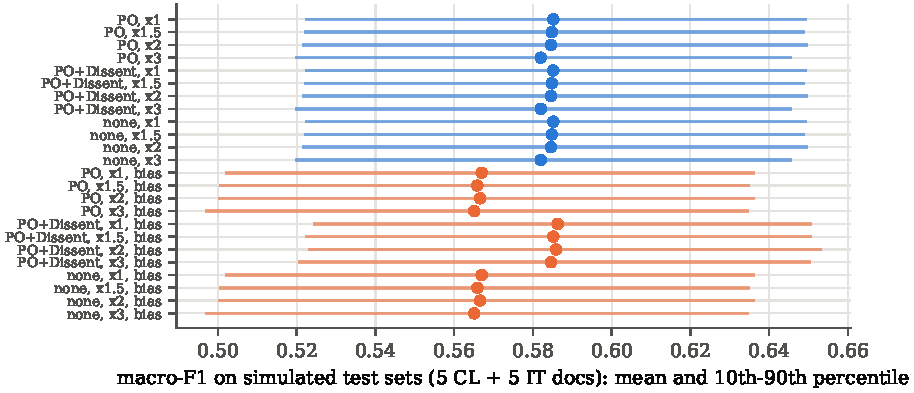
\includegraphics[width=0.9\linewidth]{figs/postproc.pdf}
\caption{C3 decoding variants on 3{,}000 simulated test sets (blocked labels: PO = PrecedentOverruled;
x = CRF transition scale; bias = calibrated per-label bias).}
\label{fig:postproc}\end{figure}

\begin{table}[H]\centering\small
\caption{C3 decoding variants: OOF macro-F1 over 90 documents, simulated-test mean and 10th--90th percentile,
predicted segments per document.}\label{tab:postproc}
\begin{tabular}{lrlrrlr}\toprule
Blocked & Scale & Bias & OOF F1 & Test-like mean & p10--p90 & Segments\\\midrule
\tabinput{tables/postproc.tex}
\bottomrule\end{tabular}\end{table}

\subsection{Submissions}
\nzips{} format-checked zips are in \code{p3/submissions/} (\autoref{tab:subs}).
\authorbox{leaderboard scores}{Add the Codabench test macro-F1 (and precision / recall) of each uploaded
submission, and say which six or more count towards the requirement.}

{\scriptsize\begin{longtable}{ll}\caption{Submission files and the run or ensemble they come from.}\label{tab:subs}\\
\toprule File & Run\\\midrule\endfirsthead\toprule File & Run\\\midrule\endhead
\tabinput{tables/submissions.tex}
\bottomrule\end{longtable}}

% =====================================================================
\section{Analysis}
\authorbox{analysis of the results}{The course rules do not allow LLM-written result analysis.  Questions the
course asks (§9.5), with the evidence above:
\begin{itemize}
  \item Which adaptation techniques work best for RR, and can parameter-efficient methods approach full
  adaptation (\autoref{tab:first}, \autoref{tab:tuning}, \autoref{fig:eff})?
  \item Does context improve sentence-level prediction (E0 vs E1)?
  \item Which roles remain hard to distinguish, and why (\autoref{fig:perlabel}, \autoref{fig:confusion})?
  \item Does performance differ between CL and IT?
  \item Does distillation keep performance while improving efficiency (E6, T13)?
  \item How do model size and compute change across experiments?
  \item Are the Phase-1 representations useful here (original vs cleaned backbone; causal vs bidirectional)?
  \item Why can a 10-document test score differ from the cross-validated estimate (\autoref{fig:postproc})?
\end{itemize}}

\section{Limitations and next steps}
Facts that limit the conclusions (the interpretation is the author's):
\begin{itemize}
  \item 90 labelled documents; fold scores vary by 0.01--0.05 (standard deviation).
  \item Several tuning decisions were made on the same out-of-fold scores they are reported on; only the
  calibration estimate is nested.
  \item One seed per run except T8, T18 and T19 (same configuration, three seeds).
  \item PrecedentOverruled (\sentsOverruled{} sentences) and Dissent (\docsDissent{} documents) have too few
  examples to be learned.
  \item Training chunks hold 128 sentences, shorter than most documents; the 512-sentence variant (T1) was not
  combined with the later changes.
\end{itemize}
\authorbox{what you would do next}{With more time or compute: \ldots}

\section{Conclusions}
\authorbox{conclusions}{Summarise what you conclude from the experiments, in your own words.}

\section{Reproducibility}
\noindent{\small\begin{tabularx}{\linewidth}{l>{\raggedright\arraybackslash}X}
First round (CV + zips) & \code{bash run\_all.sh}\\
Tuning rounds & \code{bash run\_tune.sh} (configs in \code{configs/tune*})\\
One experiment & \code{python train.py --config configs/e1\_a4\_lorma.yaml [--folds 0 2]}\\
Fold-ensemble zip & \code{python make\_submission.py --run runs/T7\_e1\_causal\_ep20\_tau05}\\
Cross-run ensemble (OOF) & \code{python ensemble\_cv.py --run runs/E1\_a4\_lorma runs/E3\_a3\_rslora --name T5}\\
Ensemble + calibration + zip & \code{python calibrate.py --run runs/T7... runs/T8... --name C1\_ens\_t7\_t8}\\
Post-processing study & \code{python postproc.py --name C3\_ens\_t7\_t8\_t10\_t9 --use-bias}\\
Comparison table & \code{python compare.py}\\
Figures and tables & \code{python p3/report/make\_figures.py}\\
\end{tabularx}}
\authorbox{repository link}{GitHub: \url{https://github.com/...}}

\section*{LLM declaration}
\authorbox{LLM declaration (mandatory)}{Fill in the course questionnaire.  Describe honestly which parts used
an LLM assistant (for example the model and PEFT code, CV/ensemble/calibration scripts, figures and this
report's methods/results text) and which parts are your own (design decisions, hyperparameters, analysis,
conclusions).}

\begin{thebibliography}{99}\small
\bibitem{bhattacharya2019rr} P.~Bhattacharya et al. Identification of rhetorical roles of sentences in Indian legal judgments. JURIX 2019.
\bibitem{bihany2025lorma} H.~Bihany, S.~Patel, A.~Modi. LoRMA: Low-rank multiplicative adaptation for LLMs. Findings of ACL 2025.
\bibitem{dettmers2023qlora} T.~Dettmers et al. QLoRA: Efficient finetuning of quantized LLMs. NeurIPS 2023.
\bibitem{hinton2015kd} G.~Hinton, O.~Vinyals, J.~Dean. Distilling the knowledge in a neural network. arXiv:1503.02531, 2015.
\bibitem{hochreiter1997lstm} S.~Hochreiter, J.~Schmidhuber. Long short-term memory. Neural Computation, 1997.
\bibitem{hu2022lora} E.~Hu et al. LoRA: Low-rank adaptation of large language models. ICLR 2022.
\bibitem{kalajdzievski2023rslora} D.~Kalajdzievski. A rank stabilization scaling factor for fine-tuning with LoRA. arXiv:2312.03732, 2023.
\bibitem{lafferty2001crf} J.~Lafferty, A.~McCallum, F.~Pereira. Conditional random fields. ICML 2001.
\bibitem{lester2021prompt} B.~Lester, R.~Al-Rfou, N.~Constant. The power of scale for parameter-efficient prompt tuning. EMNLP 2021.
\bibitem{li2021prefix} X.~Li, P.~Liang. Prefix-tuning: Optimizing continuous prompts for generation. ACL 2021.
\bibitem{liu2022ia3} H.~Liu et al. Few-shot parameter-efficient fine-tuning is better and cheaper than in-context learning. NeurIPS 2022.
\bibitem{malik2022rr} V.~Malik et al. Semantic segmentation of legal documents via rhetorical roles. NLLP Workshop 2022.
\bibitem{menon2021logit} A.~Menon et al. Long-tail learning via logit adjustment. ICLR 2021.
\bibitem{zhang2023adalora} Q.~Zhang et al. AdaLoRA: Adaptive budget allocation for parameter-efficient fine-tuning. ICLR 2023.
\end{thebibliography}
\end{document}
